
\documentclass[12pt]{article}
\usepackage{geometry}
\geometry{a4paper}


\usepackage{color}
\usepackage{hyperref}
\usepackage{amsmath}
\usepackage{amsfonts}
\usepackage{amssymb}
\usepackage{graphicx}
\usepackage{tcolorbox}
\usepackage{listings}
\usepackage{here}
\usepackage{txfonts}
\usepackage{algorithm}
\usepackage{algorithmic}
\usepackage{siunitx}
\usepackage{xcolor}

\lstset {language = c++,
  basicstyle = \ttfamily \scriptsize,
  commentstyle = \textit,
  frame = tRBl,
  framesep = 5pt,
  showstringspaces = false,
  numbers = left,
  stepnumber = 1,
  numberstyle = \tiny,
  tabsize = 2,
  keywordstyle = \bfseries \color{blue},
  stringstyle=\color{magenta},
  commentstyle=\color{red},
  morecomment=[l][\color{red}]{\#}
  showstringspaces=false, % don't mark spaces in strings
}
\newcommand{\bi}[1]{\mathbf{#1}}
\newcommand{\bs}[1]{\boldsymbol{#1}}  % bold for greek characters
\newcommand{\bbR}{\mathbb{R}}

\author{Nobuyuki Umetani}

\title{Continum Mechanics:\\ Derivatives and Conservation Laws \footnote{I initially wrote this document when I was a MSc student. I tried to keep what I learned in my mind.}}


\begin{document}
\maketitle
\tableofcontents
\section{Time Derivative}

%%%%%%%%%%%%%%%%%%%%%%%%%%%%%%%%

\subsection{Object Moving In The Space}

Let's say an object is moving in the space.
%
We consider a point that move together with that object.
%
Imagine a potato that has a small cross sign cut by a knife. 
%
The center of the cross sign move together with the potato. 
%
We call that kind of object attached point as material point $\bi{X}$.
%
Please not that sometime the material point is not specifically on an object with volume. 
%
In that case, it is just spatial point that moves around.

The coordinate of material point changes over the time, so we denote the coordinate as ${\bi{X}}(t)$ .
%
It is a bit confusing but please not that we use $\bi{X}$ as a \textit{label} of a material point while $\bi{X}(t)$ means the coordinate. 


Since the physical object does not suddenly disappear or jump (we do not consider quantum mechanical here) the $\bi{X}$ is a continuous function.
%
We denote its time derivative as $v$:
%
\begin{equation}
\frac{\partial\bi{X}(t)}{\partial{t}} = \bi{v}
\end{equation}
%

In the meanwhile, a point that does not change its location we call it as \textit{spacial point} and denote it as $\bi{x}$.
%
The position of the spacial point is constant and time independent. 
%
We also denote the coordinate of the point as $\bi{x}$


\begin{figure}[htbp!]
\centering
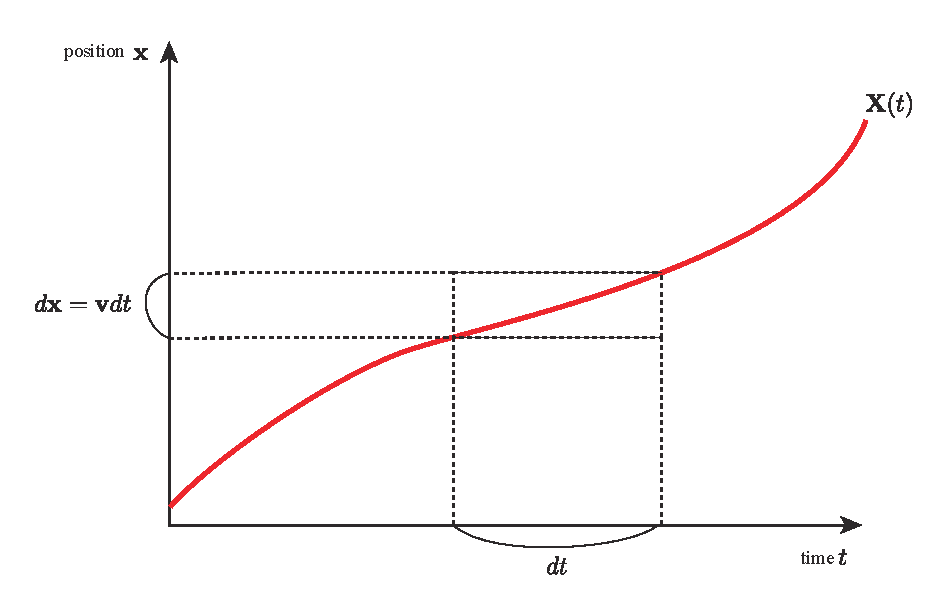
\includegraphics[width=160mm]{images/material_point.pdf}
\caption{Spatial-time visualization of the trajectory of a material point $\bi{X}$ }
\end{figure}  





\subsection{Material Time Derivative and Spatial Time Derivative}

We denote $\mathcal{A}$ as an arbitrary field that can be either scalar $a$, vector $\vec{a}$ or tensor $\bi{A}$. 
%
The word ``field" means that some value $\mathcal{A}$ is defined at some continuous region in the space (and sometimes in the time).
%
For example, in the room, there is a temperature field as you can find out the temperature at any point on the room. 
%
The corner of the room might be colder than in the middle.
%
If you put AC on, for example, the temperature dynamically changes. 



The field is defined at the point and at the time. 
%
Hence, the value of field at time $t$ and the position $\bi{x}$ can be written like a multivariate function $\mathcal{A}(t,\bi{x})$. 
%
Let's assume that this function is continuous. 
%
There is no abrupt jumping of the value $\mathcal{A}$ when I change the position or time.
%
In the math terminology, this can be said that $\mathcal{A}$ is \textit{differencible}.









The total derivative can be written as follows:
%
\begin{eqnarray}
d{\mathcal{A}}
&=&\left.\frac{\partial\mathcal{A}}{\partial{t}}\right|_{\bi{x}}dt+\left.\frac{\partial\mathcal{A}}{\partial{x_i}}\right|_{t}dx_i\\
\label{eqn:total_derivative}
&=&\left.\frac{\partial\mathcal{A}}{\partial{t}}\right|_{\bi{x}}dt+(\mathcal{A} \otimes \nabla_x) \cdot d{\bi{x}},
\end{eqnarray}
%
here $\left.\frac{\partial\mathcal{A}}{\partial{t}}\right|_{\bi{x}}$ describe how value $\mathcal{A}$ at the space-fixed position $\bi{x}$ change over time. This is called \emph{spatial time derivative}.

\begin{tcolorbox}[title=spatial time derivative]
\begin{equation}
\left.\frac{\partial\mathcal{A}}{\partial{t}}\right|_{\bi{x}}
\end{equation}
\end{tcolorbox}



\subsection{Material Time Derivative}


Here we try to obtain change of $d\mathcal{A}$ at the material point $\bi{X}$ over infinitesimal time $dt$.
%
Here, $\bi{X}$ can be seen as a label on the material point. 
%
The rate of the change in $\mathcal{A}$ on the material point $\bi{X}$ is called \emph{material time derivative} and often denoted as as:
%
\begin{tcolorbox}[title=material time derivative]
\begin{equation}
\left.\frac{\partial\mathcal{A}}{\partial{t}}\right|_{\bi{X}}
\end{equation}
\end{tcolorbox}
%




%
We plug this in the Equation~\eqref{eqn:total_derivative}.

\begin{equation}
d{\mathcal{A}}=\left.\frac{\partial\mathcal{A}}{\partial{t}}\right|_{\bi{X}}dt=\left.\frac{\partial\mathcal{A}}{\partial{t}}\right|_{\bi{x}}dt+( \mathcal{A} \otimes \nabla_x ) \cdot {\bi{v}}dt
\end{equation}

Hence we obtain following relationship between material time derivative and spatial time derivative:
%
\begin{tcolorbox}[title=relationship between material time derivative and spatial time derivative]
\begin{equation}
\left.\frac{\partial\mathcal{A}}{\partial{t}}\right|_{\bi{X}}  =  \left.\frac{\partial\mathcal{A}}{\partial{t}}\right|_{\bi{x}}+{( {\mathcal{A}} \otimes \nabla_x ) \cdot \bi{v}}
\end{equation}
\end{tcolorbox}




\begin{figure}[htbp!]
\centering
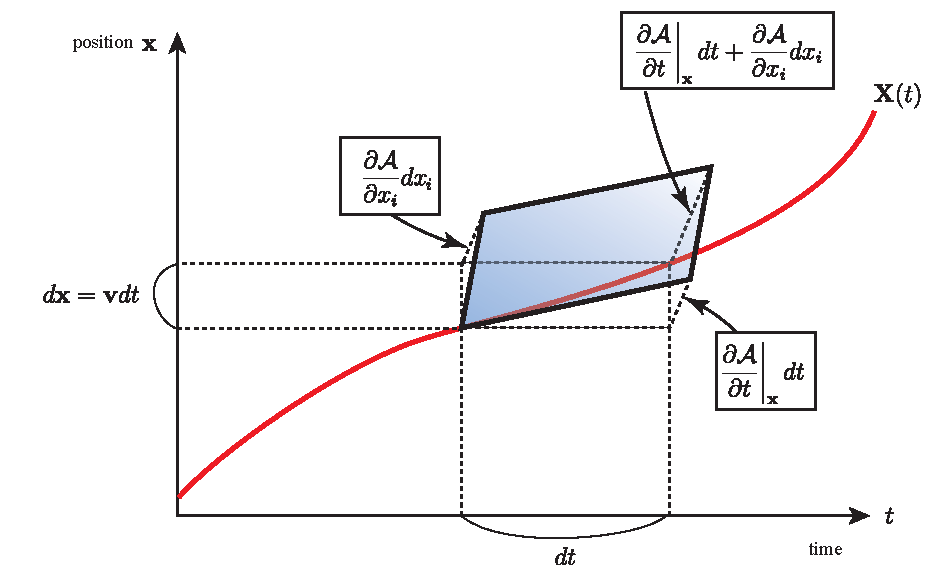
\includegraphics[width=160mm]{images/space_time_derivative.pdf}
\caption{Spatial time derivative. The axis vertical to the screen denote the value of $\mathcal{A}$.  }
\end{figure}  




\subsection{Eular's Expansion Formula}

\begin{eqnarray}
J = \det\bi{F}
\end{eqnarray}

\begin{eqnarray}
d\dot{v}  
&=&\dot{J}dV\\ 
&=&{\Big(\big[\quad d{\bi{x}_1} \quad d{\bi{x}_2} \quad d{\bi{x}_3} \quad \big]\Big)}^{.}\\  										
&=&{\Big(\big[\quad {\bi{F}} \cdot d{\bi{X}_1} \quad {\bi{F}} \cdot d{\bi{X}_2} \quad {\bi{F}} \cdot d{\bi{X}_3} \quad \big]\Big)}^{.}\\  				
&=&\left[ \quad \dot{\bi{F}} \cdot d{\bi{X}_1} \quad {\bi{F}} \cdot d{\bi{X}_2} \quad {\bi{F}} \cdot d{\bi{X}_3} \quad \right] \\
\quad && + \left[ \quad {\bi{F}} \cdot d{\bi{X}_1} \quad \dot{\bi{F}} \cdot d{\bi{X}_2} \quad {\bi{F}} \cdot d{\bi{X}_3} \quad \right]\\
\quad && + \left[\quad {\bi{F}} \cdot d{\bi{X}_1} \quad {\bi{F}} \cdot d{\bi{X}_2} \quad \dot{\bi{F}} \cdot d{\bi{X}_3} \quad \right]\\ 
&=&\left[\quad ( \dot{\bi{F}} \cdot {\bi{F}^{-1}} ) \cdot {\bi{F}} \cdot d{\bi{X}_1} \quad {\bi{F}} \cdot d{\bi{X}_2} \quad {\bi{F}} \cdot d{\bi{X}_3} \quad \right]\\
\quad &&+ \left[ \quad {\bi{F}} \cdot d{\bi{X}_1} \quad ( \dot{\bi{F}} \cdot {\bi{F}^{-1}} ) \cdot {\bi{F}} \cdot d{\bi{X}_2} \quad {\bi{F}} \cdot d{\bi{X}_3} \quad \right]\\ 
\quad && + \left[ \quad {\bi{F}} \cdot d{\bi{X}_1} \quad {\bi{F}} \cdot d{\bi{X}_2} \quad ( \dot{\bi{F}} \cdot {\bi{F}^{-1}} ) \cdot {\bi{F}} \cdot d{\bi{X}_3} \quad \right]\\ 
&=&{\rm tr}({\bi{F}^{-1}} \cdot {\bi{F}} ) \left[ \quad {\bi{F}} \cdot d{\bi{X}_1} \quad {\bi{F}} \cdot d{\bi{X}_2} \quad {\bi{F}} \cdot d{\bi{X}_3} \quad \right]\\		
&=&	({\rm tr}{\bi{L}})(\det{\bi{F}})\left[ \quad d{\bi{X}_1} \quad d{\bi{X}_2} \quad d{\bi{X}_3}\quad \right]\\
&=&(\nabla_x \cdot {\bi{v}})JdV
\end{eqnarray}

Hence the rate of change of the determinant of Jacobian can be written as:
\begin{tcolorbox}[title=Euler's expansion formula]
\begin{equation}
\label{eqn:eulers_expansion_formula}
\dot{J} = ( \nabla_x \cdot {\bi{v}})J 
\end{equation}
\end{tcolorbox}
%
This is called \emph{Eular's expansion formula}.



%%%%%%%%%%%%%%%%%%%%%%%%%%%%%%%%%%%%%%%%%%%%%%%%%%%%%%%%%%%%%%%%

\subsection{The Reynolds Transport Theorem}

We consider arbitrary region inside an object.
%
We assume that the region change its change following the velocity of material points.
%
Namely, all the material point inside this region kept contained inside region over time.
%
Such region is called \emph{material control volume}.
%
The Reynolds transport theory describe how the physical quantity $\mathcal{A}$ inside such volume change over time.
\begin{tcolorbox}[title=Reynolds transport theorem]
\begin{equation}
\label{eqn:reynolds_transport_theorem}
\left.\frac{\partial}{\partial{t}}\right|_{\bi{X}}\int_v\mathcal{A}dv  
=
\int_v \left.\frac{\partial\mathcal{A}}{\partial{t}}\right|_{\bi{x}}  dv+\int_s n_x \cdot ( {\bi{v}} \otimes \mathcal{A} ) ds
\end{equation}
\end{tcolorbox}

\begin{eqnarray}
\label{eqn:reynodls_transport_theorem1}
\left.\frac{\partial}{\partial{t}}\right|_{\bi{X}}\int_v\mathcal{A}dv  	
&=&  \left.\frac{\partial}{\partial{t}}\right|_{\bi{X}}\int_V\mathcal{A}JdV\\ 
&=&  \int_V \left.\frac{\partial\mathcal{A}}{\partial{t}}\right|_{\bi{X}}J+\mathcal{A} \dot{J} dV\\ 
&=&  \int_V \left.\frac{\partial\mathcal{A}}{\partial{t}}\right|_{\bi{X}}J+\mathcal{A}(\nabla_x \cdot {\bi{v}}) J dV\\  
&=&  \int_v \left.\frac{\partial\mathcal{A}}{\partial{t}}\right|_{\bi{X}}+\mathcal{A}(\nabla_x \cdot {\bi{v}})dv\\  
&=&  \int_v \left.\frac{\partial\mathcal{A}}{\partial{t}}\right|_{\bi{x}}+{\bi{v}} \cdot ( \nabla_{x} \otimes \mathcal{A} )+\mathcal{A}(\nabla_x \cdot {\bi{v}} ) dv \\  		
&=&  \int_v \left.\frac{\partial\mathcal{A}}{\partial{t}}\right|_{\bi{x}}+\nabla_x \cdot ( {\bi{v}} \otimes \mathcal{A} ) dv\\  
&=&  \int_v \left.\frac{\partial\mathcal{A}}{\partial{t}}\right|_{\bi{x}}  dv+\int_s n_x \cdot ( {\bi{v}} \otimes \mathcal{A} ) ds ,
\end{eqnarray}
%
where $V$ is the region in the initial configuration.

In the first line \eqref{eqn:reynodls_transport_theorem1}, the differential is computed over the time changing volume $v$ and we need to care about the rate of boundary change.
%
We make this tractable by transforming the integral domain into the reference volume $V$, which does not change over time.
Then, we again change the integration into the current volume $v$.



%このReynoldsの輸送定理を使って積分形式の式を微分形式に変換する時には、物質検査体積を任意にとれることから被積分関数における式が常に成り立つということをよく使う。


Note that we used Euler's expansion formula (Equation~\ref{eqn:eulers_expansion_formula}) and following formula about volume change from current and reference configuration:
%
\begin{eqnarray}
dv  
&=&  \left[\quad d{\bi{x}_1} \quad d{\bi{x}_2} \quad d{\bi{x}_3} \quad \right]\\  
&=&  \left[\quad {\bi{F}} \cdot d{\bi{X}_1} \quad {\bi{F}} \cdot d{\bi{X}_2} \quad {\bi{F}} \cdot d{\bi{X}_3} \quad \right]\\  
&=&  (\det{\bi{F}})\left[ \quad d{\bi{X}_1} \quad d{\bi{X}_2} \quad d{\bi{X}_3} \quad \right]\\  
&=&  JdV 
\end{eqnarray}


Using the Reynolds transport theorem, we can derive many useful equations such as the continuity equation, momentum equation, and energy equation.


%%%%%%%%%%%%%%%%
%%%%%%%%%%%%%%%%%%%%%%%%%%%%%%%%%%%%%%%%%%%%%%%%%%%%%%%%%%%%%%%%

\section{Differential form of Conservation Law}

%%%%%%%%%%%%%%%%%%%%%%%%%%%%%%%%%%%%%%%%%%%%%%%%%%%%%%%%%%%%%%%%

\subsection{Equation of Continuity}

An objects' mass $m$ is given using its shape $v$ and density $\rho$ as:
%
\begin{equation}
m=\int_v\rho dv.
\end{equation}
%

The principle of conservation of mass state that an objects mass $m$ is constant over time and unchanged with the deformation:
\begin{equation}
\left.\frac{\partial{m}}{\partial{t}}\right|_{X}  =  \left.\frac{\partial}{\partial{t}}\right|_{X}\int_v\rho dv =0 
\end{equation}



We plug-in this principle of conservation of mass into the Reynolds transport theorem by changing $\mathcal{A}$ to $\rho$ as:
\begin{equation}
\left.\frac{\partial}{\partial{t}}\right|_{\bi{X}}\int_v{\rho}dv			
=\int_v \left.\frac{\partial\rho}{\partial{t}}\right|_{\bi{X}} + \rho(\nabla_x \cdot {\bi{v}})dv
\end{equation}
Hence,
\begin{equation}
 \int_v \left.\frac{\partial\rho}{\partial{t}}\right|_{\bi{X}} + \rho(\nabla_x \cdot {\bi{v}})dv = 0 
\end{equation}
%
Since this holds in the arbitrary region $v$, we have
%
\begin{equation}
\left.\frac{\partial\rho}{\partial{t}}\right|_{\bi{X}} + \rho(\nabla_x \cdot {\bi{v}}) = 0.
\end{equation}
%
This is the Lagrangian representation of continuity equation.




\begin{tcolorbox}[title=continuity equation (Lagrangian form)]
\begin{equation}
\left.\frac{\partial\rho}{\partial{t}}\right|_{\bi{X}} + \rho(\nabla_x \cdot {\bi{v}}) = 0 
\end{equation}
\end{tcolorbox}


Further more we substitute $\mathcal{A}$ in Reynolds transport theory to $\rho$ to obtain following equation.

\begin{equation}
\left.\frac{\partial}{\partial{t}}\right|_{\bi{X}}\int_v{\rho}dv			
=\int_v \left.\frac{\partial\rho}{\partial{t}}\right|_{\bi{x}} + \nabla_x \cdot ( \rho{\bi{v}} ) dv
\end{equation}

%%%%%%%%%%%%%%%%
Since this holds in arbitrary region $v$, we have
%
\begin{equation}
\left.\frac{\partial\rho}{\partial{t}}\right|_{\bi{x}} + \nabla \cdot ({\bi{v}} \rho) = 0.
\end{equation}

This is the Eularian form of continuity equation.

\begin{tcolorbox}[title=continuity equation (Eularian form)]
\begin{equation}
\left.\frac{\partial\rho}{\partial{t}}\right|_{\bi{x}} + \nabla \cdot ({\bi{v}} \rho) = 0
\end{equation}
\end{tcolorbox}


\subsection{Special Case of Reynolds Transport Theorem where Transported Quantity is Proportional to the Density}

Let's consider a special case of transportation where the transported quantity is proportional to the density, such as momentum transportation.
%
In such a case, we can put the transport theorem in simpler form.
%
Let's say the transported quotient can be represented as $\rho\mathcal{A}$. 

\begin{eqnarray}
\left.\frac{\partial}{\partial{t}}\right|_{\bi{X}} \int_v \rho {\mathcal{A}} dv
&=& \left.\frac{\partial}{\partial{t}}\right|_{\bi{X}} \int_V \rho {\mathcal{A}} J dV\\	
&=& \int_V \left.\frac{\partial\rho}{\partial{t}}\right|_{\bi{X}} {\mathcal{A}} J	+ \rho \left.\frac{\partial\mathcal{A}}{\partial{t}}\right|_{\bi{X}} J + \rho {\mathcal{A}} \dot{J} dV\\
&=& \int_V \left.\frac{\partial\rho}{\partial{t}}\right|_{\bi{X}} {\mathcal{A}} J + \rho \left.\frac{\partial\mathcal{A}}{\partial{t}}\right|_{\bi{X}} J + \rho {\mathcal{A}} ( \nabla_x \cdot {\bi{v}} ) J dV\\
&=& \int_v \underbrace{( \left.\frac{\partial\rho}{\partial{t}}\right|_{\bi{X}} + \rho ( \nabla_x \cdot {\bi{v}} ) ) }_{=0} {\mathcal{A}} + \rho \left.\frac{\partial\mathcal{A}}{\partial{t}}\right|_{\bi{X}} dv
\end{eqnarray}


The Lagrangian description of continuity equation makes the first term of the equation zero. 
%
Finally, we could include material time derivative inside integral:
%
\begin{tcolorbox}[title=special case of Reynolds transport theorem]
\begin{equation} 
\label{eqn:special_reynolds_transportation}
\left.\frac{\partial}{\partial{t}}\right|_{\bi{X}} \int_v \rho {\mathcal{A}} dv 
= \int_v \rho \left.\frac{\partial\mathcal{A}}{\partial{t}}\right|_{\bi{X}} dv	
\end{equation}
\end{tcolorbox}

Let's investigate how the principle of mass conservation can be described using the reference  configuration.
%
We denote the density in the reference configuration as $\rho_0$
%
\begin{equation}
 {\rho}dv = {\rho_0}dV 
\end{equation}
%
Additionally the using the $dv=JdV$, we have 
%
\begin{equation}
\frac{\rho_0}{\rho} = J 
\end{equation}

%%%%%%%%%%%%%%%%%%%%%%%%%%%%%%%%%%%%%%%%%%%%%%%%%%%%%%%%%%%%%%%%

\subsection{Cauchy's First Law of Motion}

The Euler's first law of motion (conservation of momentum) has:
\begin{equation}
\label{eqn:euler_first_law_motion1}
\left.\frac{\partial}{\partial{t}}\right|_{\bi{X}}\int_v \rho {\bi{v}} dv		
=\int_v \rho {\bi{g}} dv + \int_s {\bi{t}} ds.
\end{equation}

We set $\mathcal{A}=\bi{v}$ in the the special case of Reynolds transportation theorem (Equation~\eqref{eqn:special_reynolds_transportation}) to obtain
%
\begin{equation}
\label{eqn:cauchy_first_law1}
\left.\frac{\partial}{\partial{t}}\right|_{\bi{X}} \int_v \rho {\bi{v}} dv 	
=\int_v \rho \left.\frac{\partial\bi{v}}{\partial{t}}\right|_{\bi{X}} dv.
\end{equation}

We put ${\bf{t}}={\bi{T}}^{T}\cdot{\bi{n}}={\bi{n}}\cdot{\bi{T}}$
in the left hand side of Equation \eqref{eqn:euler_first_law_motion1} and apply Gauss's divergence theorem to obtain
%
\begin{eqnarray}
\int_v \rho {\bi{g}} dv + \int_s {\bi{t}} ds
&=&\int_v \rho {\bi{g}} dv + \int_s {\bi{n}} \cdot {\bi{T}} ds \\
\label{eqn:cauchy_first_law2}
&=&\int_v \rho {\bi{g}} + \nabla_x \cdot {\bi{T}} dv.
\end{eqnarray}

We put Equation~\eqref{eqn:cauchy_first_law1} and \eqref{eqn:cauchy_first_law2} into the Euler's first law of motion (Equation~\eqref{eqn:euler_first_law_motion1}) to obtain following:
%
\begin{equation}
\int_v \rho \left. \frac{\partial {\bi{v}}}{\partial t} \right|_{\bi{X}} dv	
=\int_v \rho {\bi{g}} + \nabla_x \cdot {\bi{T}} dv 
\end{equation}
%
Since this equation is true of arbitrary region $v$, we have following \emph{Cauchy's first law of motion}:
%
\begin{tcolorbox}[title=Cauchy's first law of motion (Lagrangian form)]
\begin{equation}
\label{eqn:cauchys_first_law_motion_lagrange}
\rho \left.\frac{\partial {\bi{v}}}{\partial t} \right|_{\bi{X}}	
=\rho {\bi{g}} + \nabla_x \cdot {\bi{T}}
\end{equation}
\end{tcolorbox}
%
We change the first term of the left hand side of Equation~\eqref{eqn:cauchys_first_law_motion_lagrange} from material time derivative to spatial time derivative to obtain following~\emph{Cauchy's first law of motion in Eulerian form}:
%
\begin{tcolorbox}[title=Cauchy's first law of motion (Eulerian form)]
\begin{equation}
\rho \left.\frac{\partial\bi{v}}{\partial{t}} \right|_{\bi{x}} + \rho ( {\bi{v}} \otimes \nabla_x ) \cdot {\bi{v}} 
=\rho {\bi{g}} + \nabla_x \cdot {\bi{T}} 
\end{equation}
\end{tcolorbox}




%%%%%%%%%%%%%%%%%%%%%%%%%%%%%%%%%%%%%%%%%%%%%%%%%%%%%%%%%%%%%%%%

\subsection{Cauchy's Second Law of Motion}

According to the \emph{Euler's second law of motion} we have conservation of angular momentum
%
\begin{tcolorbox}[title=Euler's second law of motion]
\begin{eqnarray}
\label{eqn:euler_second_law_motion}
\left.\frac{\partial}{\partial{t}}\right |_{\bi{X}} \int_v \bi{x} \times \rho \bi{v} dv
=	\int_v \bi{x} \times \rho \bi{g} dv	
+ \int_s {\bi{x}} \times {\bi{t}} ds
\end{eqnarray}
\end{tcolorbox}
%
For the left hand side of this Euler's first law of motion~(Equation~\eqref{eqn:euler_second_law_motion}), we put the special case of Reynolds transport theorem (Equation~\eqref{eqn:special_reynolds_transportation}) as $\mathcal{A}={\bi{x}}\times{\bi{v}}$:
%
\begin{eqnarray}
\int_v \rho \left.\frac{\partial}{\partial{t}}\right|_{\bi{X}} ( {\bi{x}} \times {\bi{v}} ) dv
&=&\int_v \rho \big( \left.\frac{\partial\bi{x}}{\partial{t}}\right|_{\bi{X}} \times {\bi{v}} + {\bi{x}}\times\left.\frac{\partial\bi{v}}{\partial{t}}\right|_{\bi{X}} \big) dv \\
&=&\int_v {\bi{x}} \times \rho \left.\frac{\partial\bi{v}}{\partial{t}}\right|_{\bi{X}}  dv 
\end{eqnarray}
%
Note that we used relationship $\left.\frac{\partial\bi{x}}{\partial{t}}\right|_{\bi{X}}\times{\bi{v}}={\bi{v}}\times{\bi{v}}=0$.


The second term of the left-hand side of Euler's second law of motion (Equation~\eqref{eqn:euler_second_law_motion}) can be further transformed as:
%
\begin{eqnarray}
\int_s {\bi{x}} \times {\bi{t}} ds
&=&\int_s {\bi{x}} \times ( {\bi{T}^T} \cdot {\bi{n}} ) ds\\
&=&\int_s (x_i{\bi{e}_i}) \times ( T_{lj} {\bi{e}_j} n_l ) ds\\
&=&\int_s {\epsilon_{ijk}} x_i T_{lj} n_l {\bi{e}_k} ds\\
&=&{\epsilon_{ijk}} \int_s x_i T_{lj} n_l ds {\bi{e}_k}\\
&=&{\epsilon_{ijk}} \int_v \frac{\partial}{\partial{x_l}} ( x_i T_{lj} ) dv {\bi{e}_k}\\
&=&{\epsilon_{ijk}} \int_v ( \delta_{il} T_{lj} + x_i \frac{\partial{T_{lj}}}{\partial{x_l}} ) dv {\bi{e}_k}\\
&=&\int_v \left( {\epsilon_{ijk}}T_{ij}{\bi{e}_k} + ({x_i}{\bi{e}_i})\times(\frac{\partial{T_lj}}{\partial{x_l}}{\bi{e}_j}) \right) dv\\
&=&\int_v ({\epsilon_{ijk}}T_{ij}{\bi{e}_k} + {\bi{x}} \times div{\bi{T}} ) dv 
\end{eqnarray}

Let's put these equations into the Euler's second law of motion (Equation~\eqref{eqn:euler_second_law_motion}):
%
\begin{eqnarray}
&&
\int_v {\bi{x}} \times \rho \left.\frac{\partial\bi{v}}{\partial{t}}\right|_{\bi{X}}  dv 
=\int_v {\bi{x}} \times \rho {\bi{g}} dv + \int_v ({\epsilon_{ijk}}T_{ij}{\bi{e}_k} + {\bi{x}} \times div{\bi{T}} ) dv \\
&\Leftrightarrow&
 \int_v {\bi{x}} \times \underbrace{( \rho \left.\frac{\partial\bi{v}}{\partial{t}}\right|_{\bi{X}} - \rho {\bi{g}} - div{\bi{T}} )}_{=0} dv 
=\int_v {\epsilon_{ijk}}T_{ij}{\bi{e}_k} dv 
\end{eqnarray}
%
Note that we applied Cauchy's first law of motion (Equation~\eqref{eqn:cauchys_first_law_motion_lagrange}) to the first term of the left hand side. 
%1
Now we have following equation:
%
\begin{equation}
\int_v {\epsilon_{ijk}}T_{ij}{\bi{e}_k} dv = 0 
\end{equation}
Because this hods in the \emph{arbitraray} volume it should be
\begin{equation}
{\epsilon_{ijk}}T_{ij}=0.
\end{equation}
In order to this holds, it requires
\begin{equation}
T_{ij} = T_{ji}
\end{equation}
Since the Cauchy stress is symmetric, the number of independent component is six.
%
The tensor notation of this is following~\emph{Cauchy's second law of motion}.
%
\begin{tcolorbox}[title=Cauchy's second law of motion]
\begin{eqnarray}
{\bi{T}^T} = {\bi{T}}
\end{eqnarray}
\end{tcolorbox}


\if0
$\bi{x}$\\
$t$\\
$d\bi{x} = \bi{v}dt$\\
$dt$\\
\begin{equation}
\frac{\partial\mathcal{A}}{\partial{x_i}}dx_i
\end{equation}
\begin{equation}
\left.\frac{\partial\mathcal{A}}{\partial{t}}\right|_{\bi{x}} dt
\end{equation}

\begin{equation}
\left.\frac{\partial\mathcal{A}}{\partial{t}}\right|_{\bi{x}} dt 
+
\frac{\partial\mathcal{A}}{\partial{x_i}}dx_i
\end{equation}

$\bi{X}(t)$
\fi


\if0
\section{参考文献}
\subsection{Books}

|[[非線形有限要素法のためのテンソル解析の基礎>http://www.amazon.co.jp/非線形有限要素法のためのテンソル解析の基礎-久田-俊明/dp/4621045814/ref=sr_1_1/503-1037623-9010312?ie=UTF8&s=books&qid=1177860149&sr=8-1]]| 久田俊明 著|
|[[「連続体力学—簡明な理論と例題」>http://books.google.com/books?id=QSXIHQsus6UC&pg=PP1&ots=MV-TnVhVYW&dq=continuum+mechanics&sig=UH1-de4DH7k4X6T2a9d4govwnmk]]|P.チャドウィック 著|

RIGHT:Made by''' Nobuyuki UMETANI'''梅谷 信行
RIGHT:
\bibliographystyle{tipsj}\bibliography{../../main}
\fi
\end{document}
